In this project ROS software is used. It creates good and feature rich environment for simple nodes which can easily communicate to each other.

\subsection{Global picture}
The overall block diagram of the system is presented in Figure \ref{fig:global}. Each of them will be explained in more detail in the following pages.
\begin{figure}[h]    
\centering    
                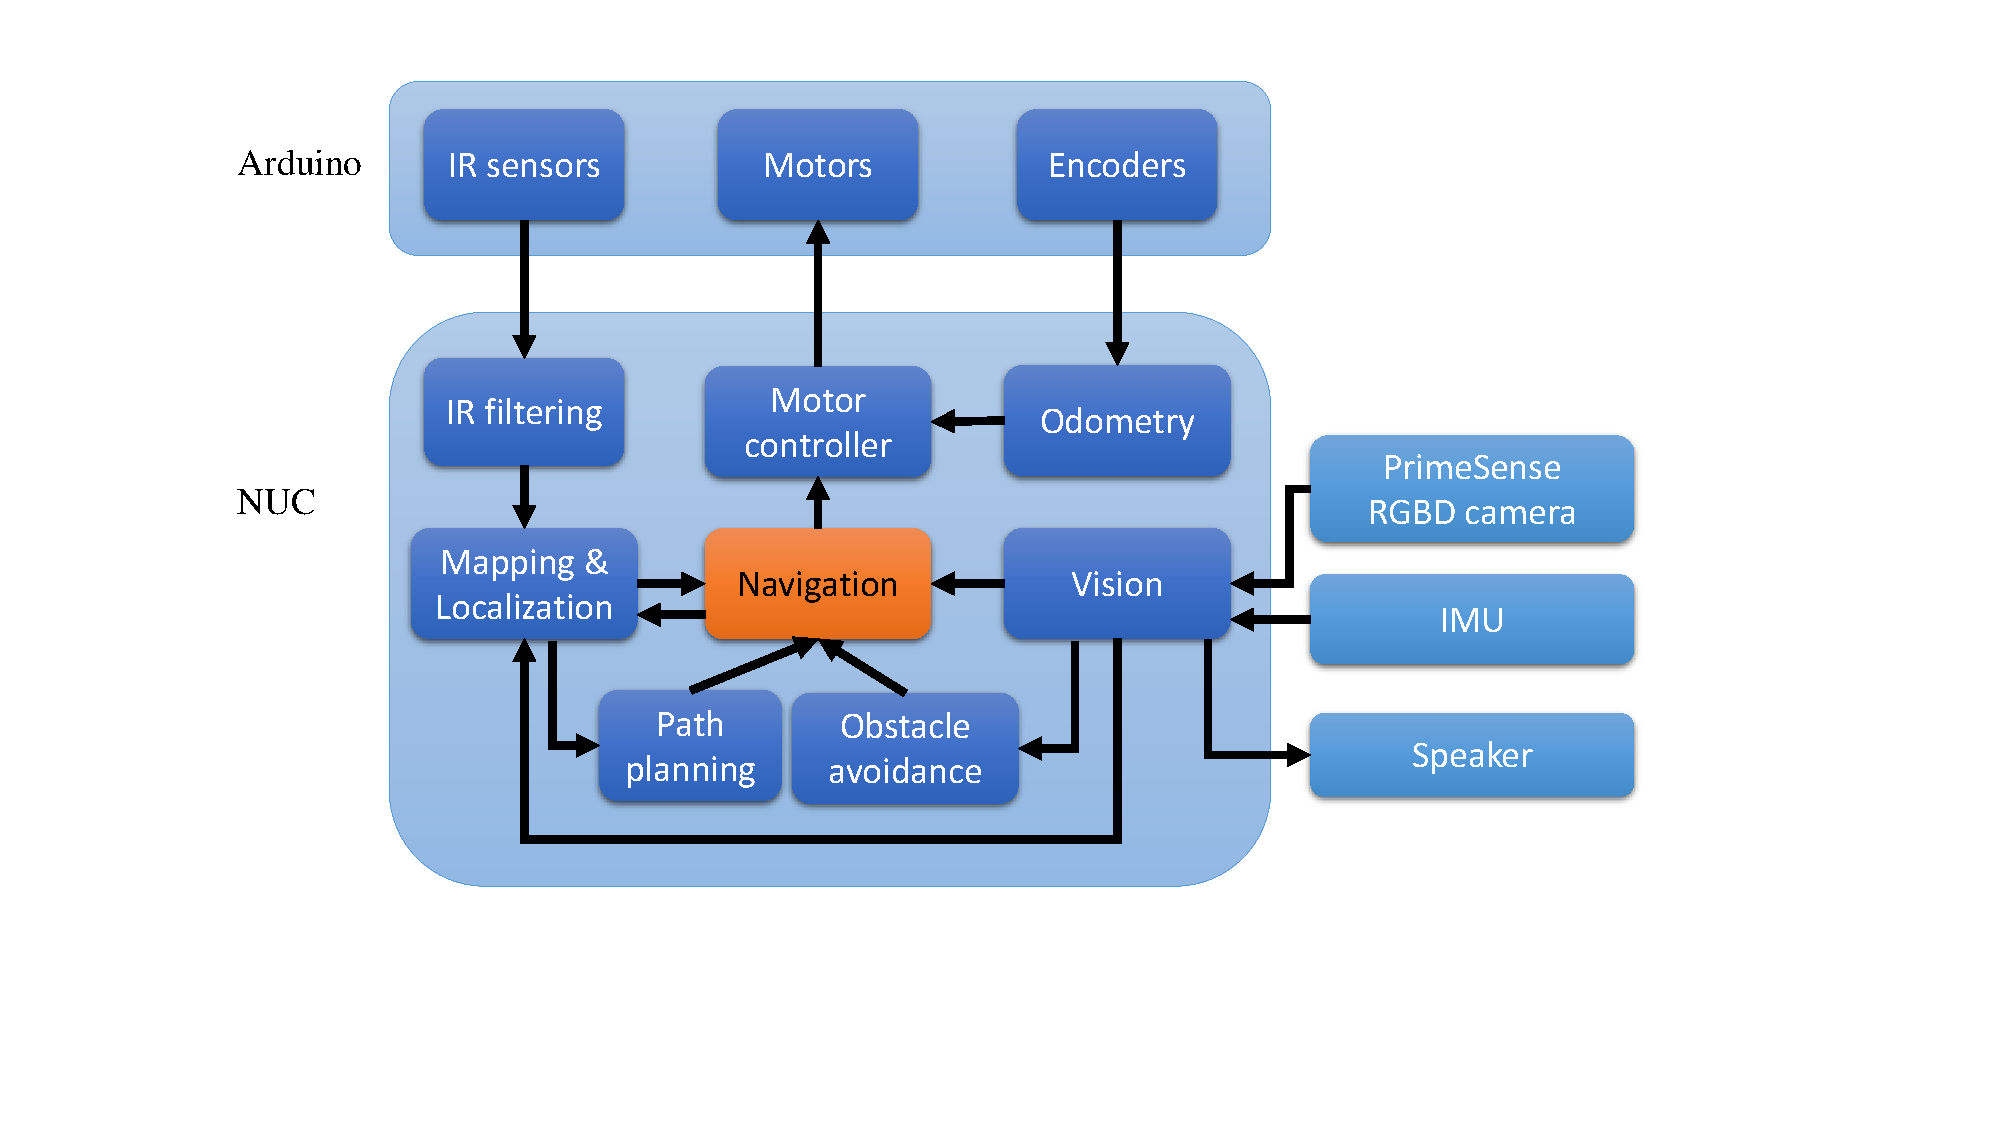
\includegraphics[trim = 0mm 40mm 60mm 0mm, clip, width=.7\textwidth]{figures/Global.pdf}
                \caption{Block diagram of the system}
                \label{fig:global}
\end{figure}
\subsection{Odometry}

Odometry node takes raw data from motor encoders and translates it into global coordinates and angle according to equations \ref{eq:odometry_eq}. This data can be used for mapping and localization. Problem with odometry is that it tends to drift especially when speed increases.

\label{eq:odometry_eq}
\begin{align}
\Delta_{l} &= \frac{2\pi \cdot R \cdot n_{l}}{M}  \\
\Delta_{r} &= \frac{2\pi \cdot R \cdot n_{r}}{M} \\
\Delta x &= \frac{\Delta_{l} + \Delta_{r}}{2} \cdot \cos(\theta) \\
\Delta y &= \frac{\Delta_{l} + \Delta_{r}}{2} \cdot \sin(\theta) \\
\Delta \theta &= \frac{\Delta_{l} - \Delta_{r}}{B}
\end{align}

, where $\Delta_l$ and $\Delta_r$ are the distance travelled by the left and right wheel, respectively, $R$ is the wheel radius (assumed to be equal for both wheels), $n_l$ and $n_r$ is the number of ticks that the corresponding has rotated, $M = 360$ is the number of ticks per revolution, $B$ is the distance between wheels and $\Delta x$, $\Delta y$ and $\Delta\theta$ is the change in robot pose in $x,y$ and $\theta$ (in global coordinates).




\subsection{Mapping}
Mapping is done in a separate node called mapping. We create 3 different maps of the same sizes. The so called raw map, the thick map, and the cost map. For the raw and thick map we chose to use the occupancy grid package from ROS. We use three distinct values that each represents the states unknown, free or occupied area. For the cost map we simply used an int array in the form of a ROS message of type Int64MultiArray.

For the raw and thick map the free cells were calculated in similar fashion. Every cell that the robot went over, gets set to a free cell, no matter the value before. All cells touched by the IR sensors on the sides, up to a certain maximum distance or up until we get an occupied reading, also gets set to free cell. All cells in between the end and start points of the 2 sensors on each side gets set to free. However these cells do not overwrite occupied cells since we are just assuming that the area is free. The reason for why this is done is to make sure we do not leave behind lonely unknown cells that can influence the path planning. Furthermore to make the path planning more stable and react faster on close walls in front of the robot, we set all cells 10 cm ahead of the robot to free cells. These also of course do not overwrite occupied cells since we have no assurance that the cells are in fact not occupied by something. 

\begin{figure}[h]
        \centering
        \begin{subfigure}[b]{0.45\linewidth}
        \centering
                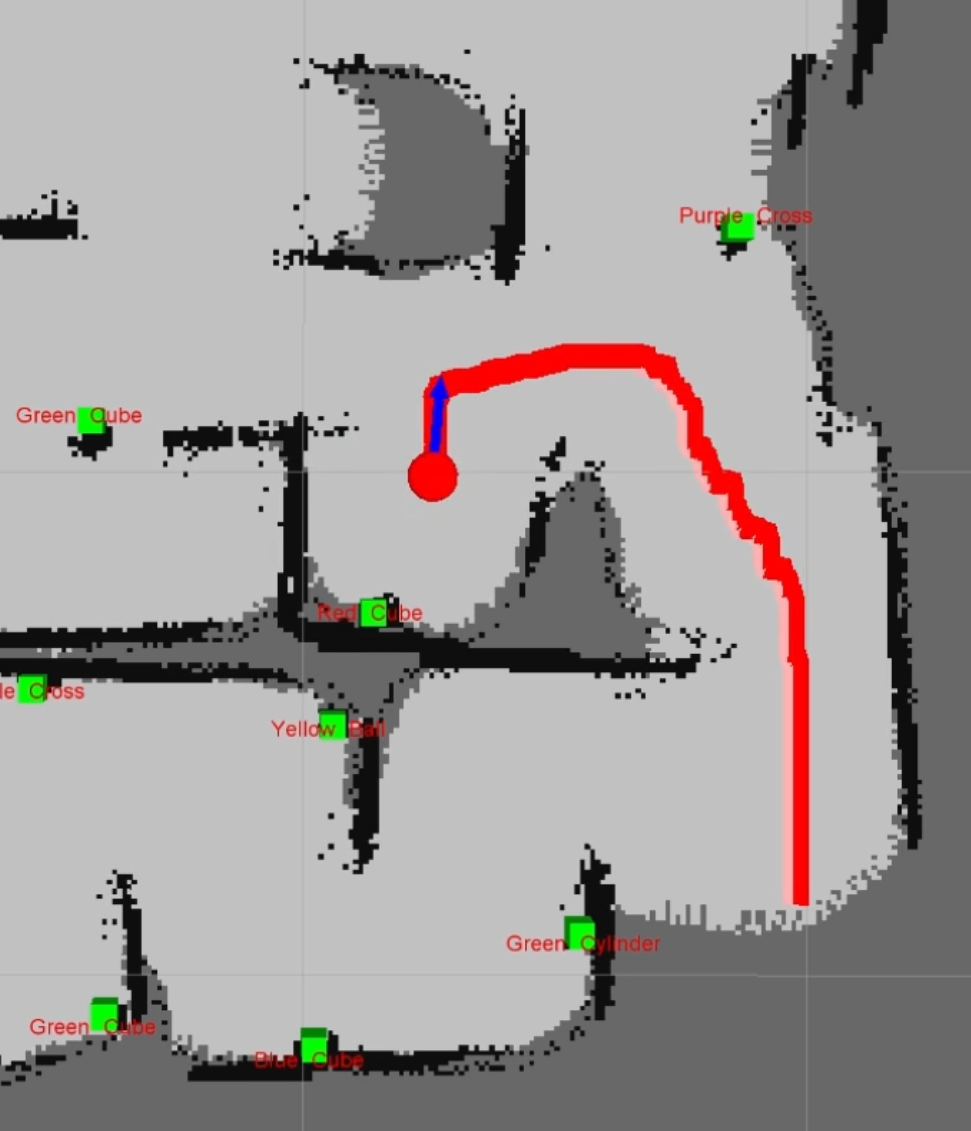
\includegraphics[height=3cm]{figures/raw_map.png}
                \subcaption{Raw map}
                \label{fig:raw_map}
        \end{subfigure}        
        \begin{subfigure}[b]{0.45\linewidth}
        \centering
                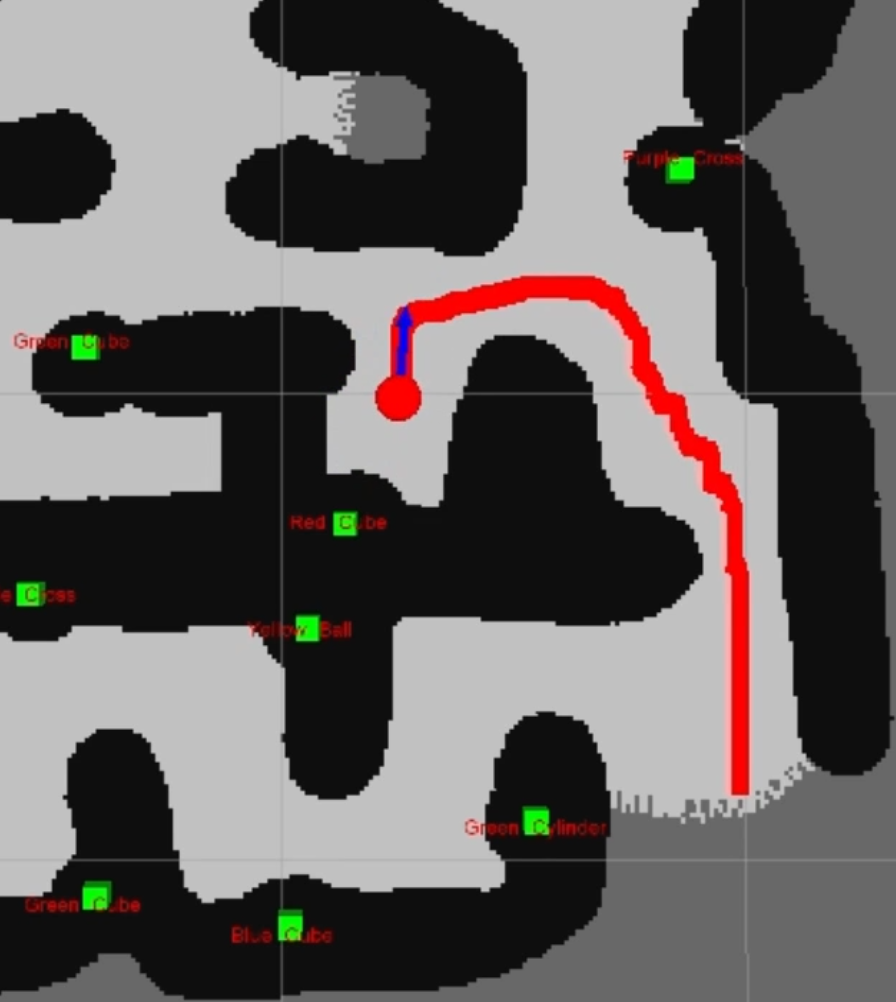
\includegraphics[height=3cm]{figures/thick_map.png}
                \caption{Thick map}
                \label{fig:thick_map}
        \end{subfigure}
        \caption{Generated maps}
        \label{fig:maps}
\end{figure}

\subsubsection{Raw map}
The raw map does no special processing when detecting occupied area. Initially all area is unknown and by driving around and getting corresponding data from IR sensors, free area and occupied area (obstacles and walls) are detected and drawn in map. The four short IR sensors on the sides of the robot provide data about distances to the walls. This data together with position information from odometry node are the basic ingredients to create the map.
We also use the laser scanner mentioned in section \ref{sec:laser} to fill occupied cells in front of the robot. And finally we use the coordinates of detected objects mentioned in \ref{sec:Object detection} to make sure we will fill cells occupied by objects. The raw map can be observed in Figure \ref{fig:raw_map}.


\subsubsection{Thick map}
The basic map, or raw map, we only use as an intermediate step in creating the processed map, also called the thick map because of how it visually looks. The reason for this maps existence is that the data from the sensors is quite noisy, therefore some processing is needed to mitigate the noisy results and also to build a more solid map to be used for path planning. Compare Figure \ref{fig:raw_map} with Figure \ref{fig:thick_map}.

Our first approach to minimize the noise and the gaps in the wall was the following:

\begin{enumerate}
\item For each IR sensor, if that sensor detects something, save the corresponding coordinate.
\item When a sensor once again detects something. Compute the distance to the previously saved coordinate.
\item If the computed distance is lower than a certain threshold, we fill every cell in between these points as occupied cells. If not, then we just throw away the saved point.
\item The second coordinate retrieved now becomes the saved coordinate in step 1.
\item Repeat steps 2-4.
\end{enumerate}

The main problem with this method was that depending on the threshold we either got too many gaps in the map, especially at corners, or we got noisy lines that impacted the path planning too much. We tried several different works around for this, both for limiting the noise and gaps and for reducing the negative impact on path planning. But the solutions were simply not good enough and quickly became complex. We replaced this method with another method that works as follows:

\begin{enumerate}
\item When an IR sensor detects something, each cell within a certain threshold, 11 cm in our final setup, gets some value increased by one. 
\item It is not until the value of a cell reaches a certain threshold, 7 in our final setup, that it becomes an occupied cell. 
\item If the value should drop below 7, it would turn back into a free cell.
\item Repeat steps 1-3. 
\end{enumerate}

This worked really well for both noise cancellation and for creating solid occupied area. The reason is that in order to get noisy data, we would need at least 7 noisy coordinates within a 10 cm area instead of having just 2 bad readings in close proximity like with the first method. Also, since all points are stored in the map and none removed, we rarely create a gap in the walls. The main reason for the choice of 11 cm in step 1 is that this results in the walls bulking out roughly 12 cm, see Figure \ref{fig:thick_map}. This is about half the robots width so as long as the robots center position is at a free cell, it would theoretically never hit a wall. This method also made it easy to update the map, or repainting, since we only change some values around a cell in the thick map when repainting that cell in the raw map. 


\subsubsection{Cost map}
The cost map was created for the path planner to be able to create a path that tries to stay at some distance away from the walls. Without it the path planner would simply take the shortest possible path which would greatly increase the risk of crashing. One might initially think that you could just increase the threshold of 11 cm in the thick map. However, that leads to an increased risk of accidentally filling a entrance completely because of noise. So the cost map can be seen as a complementary map to the thick map. The cost map is created in similar fashion as a potential field where the only thing that changes the cost, or potential, of each cell are the occupied cells in the thick map. It works similarly as the chosen method for the thick map but instead of reacting to occupied cells in the raw map, it reacts on occupied cells in the thick map. So when an occupied cell is added, each cell within some threshold, 20 cm in our final setup, gets its cost increased. The only difference is that we increase the cost the most closests to the occupied cell in question, and the least at the distance of 20 cm. Initially the cost was calculated using the raw map but that led to a quite unfair distribution of cost. This was because the raw map could have large relative differences in compactness of occupied cells at different wall segments. 

An important detail is that the cost distribution must be non-linear. If it was linear, all free cells in between occupied area would roughly get the same value. In our robot, we chose the exponential value 1.5 that simply worked well enough. There are several other parameters that could be mentioned, for example the default value that the cells have before any cost is applied. A too low default value results in that cells that are within range for some cost distribution might rarely be considered for the path planner, which in turns leads to poorly chosen routes. A too high value results in that the path planner does not care about the cost at all, since it is roughly the same. However, to get the cost map to work we just needed a somewhat even non-linear distribution. 


\subsection{Navigation}
For navigation the navigation node was created. We wanted to be able explore the entire maze and first we tried using wall following together with a topological map but later changed to path planning. 

\subsubsection{Wall following}
The setup was quite straight forward. We tuned 3 PID’s. One was simply for following the wall. The other was for keeping a certain distance to a wall. The third was to turn as close as possible to 90-degrees. Everything actually worked pretty great and we had this setup for the first milestones. However when we started building the topological map we realized that it will be very hard to try to explore the entire maze. Questions started to arise such as how will we handle large open areas? How to deal with multiple entrances next to each other that are only separated by a slim wall segment? We realized that this might get quite complex quickly. So we chose to disband this form of navigation in favor of a more general solution.

\subsubsection{Path planning}
The path planner has a separate node since it can take up to 1 second to compute the path on a maze of size 16 $\text{m}^2$. The path planner is essentially a greedy best-first search trough the cost map and thick map. How the path planner finds a path to a unknown looks as following:

\begin{enumerate}
\item Start the greedy best-first search from the robots front position using the cost map.
\item Never accept a step into an occupied cell in the thick map.
\item Expand the search until you hit a cell with the status unknown.
\item Redo the search from the robots center position until we hit the cell found in step 2.
\item Return the path as a sequence of cells.
\end{enumerate}

The reason for the first search is that want to give some priority for finding unknown cells in front of the robot. The second search is because we want the path to origin from the center of the robot. Step 3 actually uses the second functionality of the path planner. That is to go from point A to point B. When we try to navigate using a path given by the path planner we have several procedures to select a certain point in the path and then we calculate the angle to that point and try to align the robot to that angle.

\subsubsection{Global path planning}
The global path planning consists on determining the fastest sequence of objects to be visited. This is applied in Phase 2 during the contest. 

This is a classical formulation of the Travelling Salesman Problem (TSP). Here the objects can be considered as nodes within a graph and edges that connect them with some cost.

In our particular case, we propose the following formulation:
\begin{itemize}
\item The nodes are \textbf{not} the object's position, but the position from which the robot first saw the object instead. This is done to make the path planning easier: since the objects are commonly really close to walls, we might not even find a path to them considering that it is computed is the "thickened" map. 
\item The cost between two objects is measured in terms of the \textbf{travel distance}, measured as the size of the path computed from running a Best-First Search from one object to another. This metric is much better than just using the Euclidean Distance between objects (for example, consider the case where the objects are separated by just a wall but the robot cannot go through that wall and has to turn around instead). Even a more accurate metric would include an additional cost for turning, but we did not include this in our formulation.
\end{itemize}

Therefore, after Phase 1 we can create a high-level graph connecting all the object's positions with the associated costs. 

\textbf{Solution: Genetic Algorithm}\\
Once the TSP problem, we find the best solution for it. A very elegant solution to solve is to use a Genetic Algorithm (GA) \cite{genetic}, which we apply to this particular problem. The main advantages for this is that it is simple to implement and understand, really scalable and offers a good trade-off between computational time and optimality. 

The mechanism behind the GA is quite common and the reader is referred to \cite{genetic} to get more details about it. We will mention here the relevant details:
\begin{itemize}
\item \textbf{Codification}. Genetic algorithms work with strings of chromosomes, so we need to somehow encode the graph information into a string. For this, we gave an integer ID number to each of the nodes, and formed a string as a sequence of IDs.
\item \textbf{Fitness function}. It determines the performance of a single individual from a generation. We choose the fitness of individual $i$ to be:
\begin{align}
f(i) = \left[\sum_{i = 1}^{N-1} C(i,i+1)\right]^{-1}
\end{align}
, where $C(i, i+1)$ is the travel cost of going from node $i$ to node $i+1$, and $N$ is the total number of nodes.
\item Parameters. 
\begin{itemize}
\item Number of generations: 2000.
\item Number of individuals per generation: 100
\item Number of ellite individuals: 2
\item Cross-over probability: 0.7
\item Mutation probability: 0.05
\end{itemize}
\end{itemize}

This implementation gave excellent results, with nearly optimal solutions under a reduced time (around 1.0 s on the NUC). 
\subsubsection{Exploration, phase 1}

The abstract view of the exploration phase is quite simple. It looks like following:

\begin{enumerate}
\item Set path planner to search for unknown area.
\item Follow the path.
\item Purge points along the path that we have already passed by checking what point in the path we are closest to at the moment.
\item If we receive information about an object detected at some coordinate. Change path planner to look for a path close to this object for easier object classification. Once the path has been traveled, set the path planner to continue to search for unknown area.
\item Repeat steps 1-4 until the path planner starts sending empty paths. 
\item Change path planner to look for a path towards coordinate (0,0), aka. go home.
\item Stop when home.
\end{enumerate}

Under the hood we obviously do a lot more but these are the core elements. For instance when following the current path that we have, we try to go towards the point in the path that is as far away from the robot as possible where the line between the robots center position and the point in question does not come within a certain distance from a occupied node. This makes sure that the robot does not rapidly change direction just because the path changes a lot locally. 

\subsubsection{Retrieving objects, phase 2}

This is the abstract view of phase 2 where we try to retrieve the objects:

\begin{enumerate}
\item Retrieve the list of object positions as a queue, that was stored in a certain order according to the global path planner.
\item Pop the next object position and set the path planner to find this position.
\item Follow the path.
\item When reached within a certain threshold, stop.
\item Turn the robot against the object for easier recognition and stop for a short amount of time.
\item Repat steps 1-5 until the queue is empty.
\item Change the path planner to look for a path towards coordinate (0,0), aka. go home.
\item Stop when home.
\end{enumerate}

Because of problems with localization we had a hard time running phase 2 succesfully since it would eventually crash into a wall because of drift.

\subsection{Localization}
Given the lack of time for the project, it was not possible to achieve a fully working localization module, which was really an impediment for running Phase 2. The following solutions were tested.

\subsubsection{EKF Localization}
Following the theory from the Applied Estimation course \cite{Applied}, we found out that a good solution was to use an Extended Kalman Filter \cite{Thrun} to solve this problem. It would use as input $u$ the data from the encoders, and the measurements would come from a \emph{range-and-bearing} sensor, which provides the distance and angle to a recognized object in the map relative to the robot.

The implementation followed the instructions in \cite{Applied}, but the results were not so good. A really large process noise ($Q$) and really low measurement noise ($R$) was required to notice some updated in the position. However, we discarded this idea when we realized that the localization could be non-unique: the same $\theta$ and $\rho$ could be obtained at any position on a circle of radius $\rho$ around the object, given a proper orientation for the robot. In addition, the object's position would not be stable enough to heavily rely on this information. 

\subsubsection{Orientation correction}
A solution which did work was to compute the actual orientation of the robot from it's orientation with respect to the wall. 

From this, the difference in angle, $\Delta\theta$, can be computed as:
\begin{align}
\label{eq:locTheta}
\Delta\theta = \tan^{-1}\left(\frac{d_2 - d_1}{D}\right)
\end{align}

, where $d_1$ is the front sensor and $d_2$ is the back sensor on either side of the robot, and $D$ is the separation between those sensors. 

Finally, we assume the robot has an orientation $\theta0 \in \{-\pi, -\pi/2, 0, \pi/2, \pi\}$, so the final pose estimate is given by: $\theta = \theta0 + \Delta\theta$.

This was applied when starting the robot and it worked pretty well; however this could not be applied afterwards since wall following or 90-degree turning were not used in the end in favour of just path following.  

\subsubsection{On-line localization}
Finally, we implemented a promising idea for localization, but we did not have the time to test and debug it properly. The algorithm is as follows:

\begin{itemize}
\item The current pose estimate ${x_0, y_0, \theta_0}$ and a map (occupancy grid) are given.

\item The orientation ($\theta$) is updated according to the previous section.

\item We define a search region around the current pose estimate in X and Y coordinates (e.g.: a square of $10\times10$ cm.
\item Every position $\{x,y\}$ inside that region (within some discretization margin) is assigned a cost based the current sensor readings and the map, according to Equation \ref{eq:localization}.
\begin{align}
\label{eq:localization}
J(x,y) = \sum_{i = 1}^6 (z_i - \hat{z}_i)
\end{align}
, where $z_i$ is the current sensor reading for the $i$th sensor reading, and $\hat{z}_i$ is the \emph{expected} sensor reading from the position $\{x,y\}$. This is done by raycasting from every sensor position to the saved map.

\item The new position is updated as follows:
\begin{align}
\{x,y\} = \arg\max_{x,y}J(x,y)
\end{align}

\end{itemize}


This approach would give the optimal robot position assuming that the saved map was perfect and we were given perfect sensor readings. Unfortunately this was not the case. In addition, another challenging question is when to run this procedure. Ideally, it would be better to run it after 90-degree turns, but again that was not used in the robot anymore. We are confident that a little bit more time to improve this and test would have probably resulted in satisfactory results.

